%************************************************
\section{The Agent} % (fold)
\label{sec:the_agent}
%************************************************
The agent is the active entity the simulation user can control, using various input mechanisms, in order to interact with the environment. In 3D games and simulations, there are two main graphical perspectives employed to interact with the environment -- the first-person and third-person perspectives. These perspectives are the result of positioning the camera in a certain manner, providing a different perception of the environment. To control the agent's position and orientation, the camera's position and direction are coupled to a set of input controls. As the camera is moved and rotated, it creates the impression of interaction with the 3D environment. For a more realistic interaction, various animations are carried out.

\subsection{First-Person}\label{subsec:first_person}
The first-person view is a graphical perspective rendered from the viewpoint of the agent. Figure \ref{fig:fps} illustrates the first-person view from a running simulation built with Tatus \cite{o2005testbed}.

\begin{figure}[H]
	\centering
	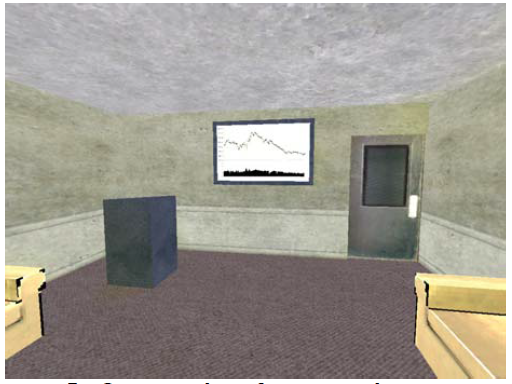
\includegraphics[width=\linewidth]{gfx/Chapter3/fps}
	\caption{A first-person perspective}
	\label{fig:fps}
\end{figure}

Using this perspective, the simulation displays what the simulation user would see with the agent's own eyes thus, objects have to be scaled accurately to appropriate sizes. It doesn't deserve a paragraph by itself.\\

In this perspective, the simulation users typically cannot see the agent's body, although it might be helpful for the user to see the agent's hands. On the plus side, there is no need for sophisticated animations for the agent, which reduces development time. Also, it helps for easier, more realistic aiming (pointing at objects to interact with) since there is no representation of the avatar to block the simulation user's view. Not seeing the agent's body reduces development efforts, but might represents a drawback as well.\\

\subsection{Third-Person}\label{subsec:third_person}
The third-person view is a graphical perspective rendered from a fixed distance behind and slightly above the virtual agent. The third-person perspective can provide an animated, strong characterized agent, directing the simulation agent's attention as she/he were watching a film.\\

On the plus side, the third-person perspective allows the simulation user to see the area surrounding the agent more clearly. This viewpoint facilitates more interaction between the virtual agent and their surrounding environment.\\

As a drawback, the third-person perspective can interfere with accurately pointing at objects, as the agent's body might block the simulation user's view. Moreover, implementing this perspective takes a lot more effort as the there is a need for an animated agent body and for custom code to make the camera follow the agent within the simulation.\\

\subsection{Discussion}\label{subsec:agent_discussion}
Based on the preceding review of existing perspectives, we have decided to include in our design a first-person perspective for the agent. An argument for choosing this perspective is that a first-person view provides the simulation user with greater immersion into the simulated environment.\\

Avatar based games and simulations usually provide both views, with an easy way to switch perspectives during runtime. For this project, a third-person perspective could be useful for future work if we are to represent wearable devices. Also, it enables the simulation user to observe the various body gestures the agent is doing.\\

To fully support requirement \ref{us:4}, we need to define a way of controlling the agent. Most games and simulations use a combination of the keyboard and the mouse to control the agent. The standard control combination is described bellow:
\begin{itemize}
	\item moving \emph{the mouse} controls the agent's direction; hence mouse movements translate into rotating the agent's viewpoint within the environment. This control is used to look around and to point at objects the simulation user desires to interact with
	\item clicking \emph{the left mouse button} triggers an interaction. The interaction is contextual; for example, clicking on a switch will turn on or off the switch. If the user clicks on a pen, the agent would pick the pen up, while if the user clicks on a surface while the agent is carrying a pen, the agent will put the pen onto the surface. Of course, the ability to carry out these actions depends on the distance between the object and the agent.
	\item moving the agent is done by activating a set of four keys on the keyboard. We have chosen the standard W, A, S, D key combination. Each key move the agent towards a certain direction, Therefore, W - forward, A - left, D - right, S - backward.
\end{itemize}

To help the simulation agent with the task of accurately aiming at objects, a cross icon will always be present in the middle of the screen. The object currently pointed at will represent the object the user intends to interact with.\\

In order to determine the object to interact with, we use the concept of \ref{ray_casting}. To achieve this, we cast a ray of infinite length from the current location of the camera along it's direction. This ray passes right through the middle of the cross and intersects all the objects along the way. We then determine the object to interact with by picking the closest object to the agent; that is the first object intersected by the ray. Moreover, the object can be interacted with only if it carries Ego metadata, otherwise the interaction is not possible. We have imposed this constraint because without the meta-data we cannot take concrete decision on what to do with the object.\\

Whether an object can be interacted with or not, is given by the current distance towards that object. Therefore, the distance has to be at most equal to the value of the ACTION\_DISTANCE property in the in the metadata.\\

Finally, the agent should not be able to pass through walls and other physical objects. Game engines provide various mechanisms for collision detection that can be used in the implementation to accommodate this aspect.\\
% section the_agent (end)